% Document class and font size
\documentclass[a4paper,10pt]{extarticle}

% Packages
\usepackage[utf8]{inputenc} % For input encoding
\usepackage{geometry} % For page margins
\geometry{a4paper, margin=0.75in} % Set paper size and margins
\usepackage{titlesec} % For section title formatting
\usepackage{enumitem} % For itemized list formatting
\usepackage{hyperref} % For hyperlinks
\usepackage{kotex}
\usepackage{graphicx}
\usepackage{array}
\usepackage{longtable}

% Formatting
\setlist{noitemsep} % Removes item separation
\titleformat{\section}{\large\bfseries}{\thesection}{1em}{}[\titlerule] % Section title format
\titlespacing*{\section}{0pt}{\baselineskip}{\baselineskip} % Section title spacing
\graphicspath{{../pictures}}

% Begin document
\begin{document}
% Disable page numbers
\pagestyle{empty}
% Enable page numbers
% \pagenumbering{arabic}

% Header

% \begin{minipage}{\textwidth}

\begin{minipage}{0.1\textwidth}
    \begin{flushleft}
        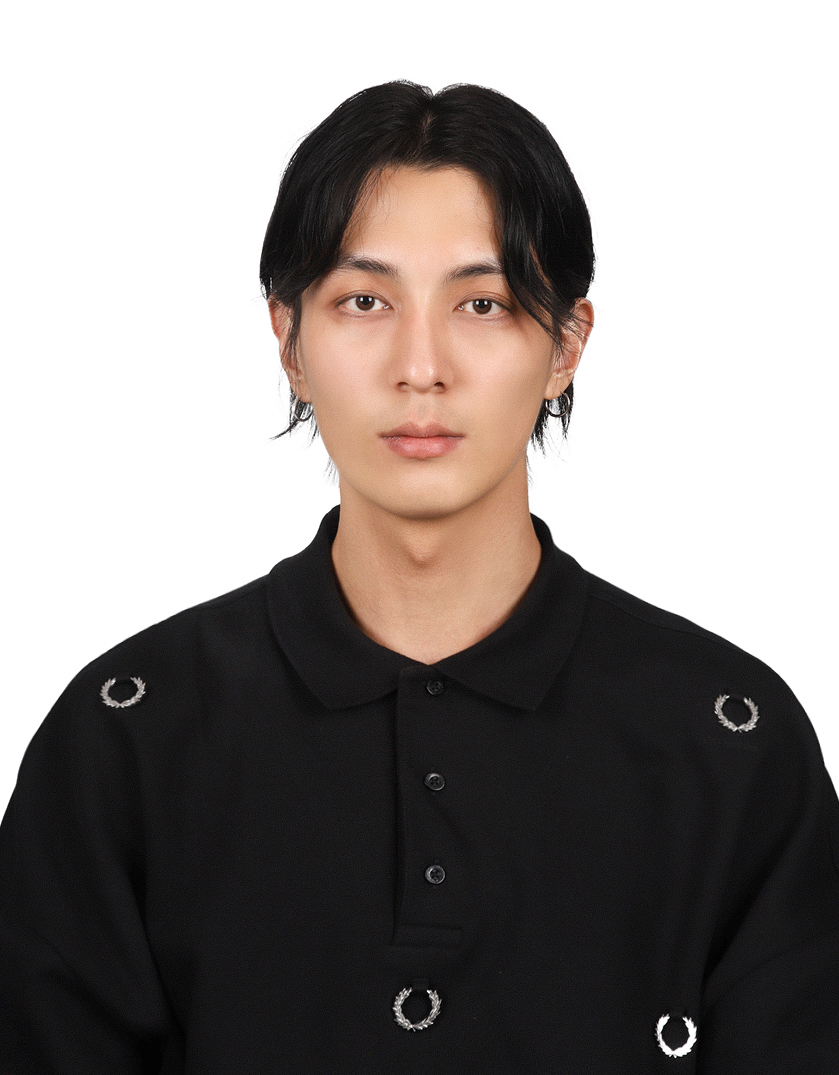
\includegraphics[height=3.5cm]{photo_231008.jpeg}
    \end{flushleft}
\end{minipage}
\hfill
\begin{minipage}{0.7\textwidth}
    \begin{flushright}
        \textbf{\Large 이현빈, Hyeonbeen Lee} % Name
        \newline\newline
        \begin{tabular}{rl}
            \textbf{Mobile: }    & +82-10-6236-4693                                                                                     \\
            \textbf{EMail: }     & \href{mailto:david.hyeonbeen.lee@gmail.com}{david.hyeonbeen.lee@gmail.com}                           \\
            \textbf{Instagram: } & \href{https://www.instagram.com/leehyeonbeen}{@leehyeonbeen}                                         \\
            \textbf{LinkedIn: }  & \href{https://www.linkedin.com/in/hyeonbeen-lee-239500286/}{linkedin.com/in/hyeonbeen-lee-239500286} \\
            \textbf{GitHub: }    & \href{https://github.com/hyeonbeenlee}{github.com/hyeonbeenlee}                                      \\
        \end{tabular}
        % \end{center}
    \end{flushright}

\end{minipage}
% \end{minipage}


% Education Section
\newcolumntype{L}{>{\raggedright\arraybackslash}m{1.6cm}}
\newcolumntype{R}{>{\centering\arraybackslash\small}m{3cm}}
\renewcommand*{\arraystretch}{1.5}
\noindent
\section*{인적사항}
\begin{center}
    \vspace*{-0.8cm}
    \noindent
    \begin{longtable}{LRLRLR}
        \textbf{성명:}   & 이현빈                                      & \textbf{생년월일:} & 1996.07.04 (양력)       & \textbf{경력여부:} & 신입       \\
        \hline
        \textbf{병역사항:} & 해병병장 만기전역 \small{(2017.05$\sim$2019.02)} & \textbf{주소:}   & 서울특별시 서초구 사임당로17길 116 & \textbf{지원분야:} & {신입 스태프} \\
        \hline
    \end{longtable}
\end{center}


% \textbf{성명}, 과학중점과정 \hfill 입학: 2012.03 | 졸업: 2015.02
% \newline
% \textbf{경희대학교}, 기계공학과 \hfill 입학: 2015.03 | 졸업: 2022.02\\ % University name and location
% 학사학위 (학위지도교수: 정신규, 김진균)\hfill 전체학점: 3.87/4.5 | 전공학점: 3.84/4.5\\ % Degree and GPA
% 학위논문명: \textit{\small{Data-driven aerodynamic coefficient prediction using}}\\
% \hspace*{1.9cm}\textit{\small{deep neural
%         network and PARSEC airfoil parameterization}}


% Education Section
\section*{학력사항}
\noindent
\textbf{반포고등학교}, 과학중점과정 \hfill 입학: 2012.03 | 졸업: 2015.02
\newline
\textbf{경희대학교}, 기계공학과 \hfill 입학: 2015.03 | 졸업: 2022.02\\ % University name and location
학사학위 (학위지도교수: 정신규, 김진균)\hfill 전체학점: 3.87/4.5 | 전공학점: 3.84/4.5\\ % Degree and GPA
학위논문명: \textit{\small{Data-driven aerodynamic coefficient prediction using}}\\
\hspace*{1.9cm}\textit{\small{deep neural
        network and PARSEC airfoil parameterization}}
\newline
\textbf{경희대학교 대학원}, 기계공학과 융합공학전공 \hfill 입학: 2022.03 | 졸업: 2024.02\\ % University name and location
석사학위 (학위지도교수: 김진균) \hfill 전체학점: 4.33/4.5\\ % Degree and GPA
학위논문명: \textit{\small{Composite neural network with differential propagation}}\\
\hspace*{1.9cm}\textit{\small{for modeling impulsive nonlinear dynamic systems}}

\section*{역량}
\begin{itemize}
    \item \textbf{영어: }학술, 비즈니스, 일상 회화 및 작문 가능
    \item \textbf{일본어: }일상 회화 가능
    \item \textbf{프로그래밍: }Python, Docker, Linux, Git, \LaTeX, MATLAB, C\#, C++, ROS
    \item \textbf{머신러닝 및 데이터분석:} PyTorch, TensorBoard, Pandas, OpenCV, Torchvision
\end{itemize}


% Experience Section
\section*{출판}
\noindent
\begin{enumerate}[leftmargin=.5cm]
    \item S. Han, G.E. Jeong, \textbf{H. Lee}, W.S. Choi, J.G. Kim, “Multi-body dynamics model for spent nuclear fuel transportation system under normal transport test conditions”, \textit{Nuclear Engineering and Technology} (IF=2.817), accepted.
    \item \textbf{H. Lee}, S. Han, H.S. Choi, J.G. Kim. “cNN-DP: Composite neural network with differential propagation for impulsive nonlinear dynamics”, \textit{Journal of Computational Physics (IF=4.645)}, submitted.
    \item \textbf{H. Lee}, J. Han, T. Yeo, J.G. Kim. “Multi-horizon force components forecasting of ocean robot using interpretable Transformer and experimental measurements”, in preparation.
\end{enumerate}

% Experience Section
\section*{학회}
\noindent
\newcolumntype{L}{>{\raggedright\arraybackslash}m{3.4cm}}
\newcolumntype{R}{>{\raggedright\arraybackslash}m{13.2cm}}
\vspace*{-.5cm}
\begin{longtable}{LR}
    {2022.12.04 \linebreak 제주시, 대한민국}           & \textbf{H. Lee}, S. Han, G.E. Jeong, J.G. Kim. “Development of multibody dynamics trailer model using normal transportation test data and DNN based surrogate model generation”, 한국소음진동공학회 (구두발표). \\
    {2023.02.16 \linebreak  Austin, Texas, USA} & \textbf{H. Lee,} S. Han, H.S. Choi, J.G. Kim. “Composite neural network framework for modeling impulsive nonlinear dynamic responses”, IMAC-XLI (구두발표).                                            \\
    {2023.03.23 \linebreak 제주시, 대한민국}           & \textbf{H. Lee,} S. Han, H.S. Choi, J.G. Kim. “Meta-modeling of nonlinear impulsive dynamics using composite neural network model with differential propagation”, 대한기계학회 신뢰성 부문 학회 (구두발표).         \\
    {2023.05.18 \linebreak 부산광역시, 대한민국}         & \textbf{H. Lee,} S. Han, H.S. Choi, J.G. Kim. “Meta-modeling of nonlinear impulsive dynamics using composite neural network model with differential propagation”, 대한기계학회 신뢰성 부문 학회 (구두발표).         \\
    {2023.11.01 \linebreak 인천광역시, 대한민국}         & \textbf{H. Lee}, J. Han, T. Yeo, J.G. Kim. “Real-time multi-horizon reaction force forecasting of ocean robot using interpretable Transformer”,  대한기계학회 본부학술대회 (구두발표).                             \\
\end{longtable}


% Experience Section
\section*{프로젝트}
\noindent
\newcolumntype{L}{>{\raggedright\arraybackslash}m{3cm}}
\newcolumntype{R}{>{\raggedright\arraybackslash}m{14cm}}
\vspace*{-.5cm}
\begin{longtable}{LR}
    {2021.09 | 2022.10} & Development of ground·sea transportation test simulation model using multibody dynamics and DNN-based metamodel, 한국원자력연구원.                                                                                                                                                                    \\
    {2021.09 | 현재}      & Metamodel generation and evolution procedures for flexible multibody dynamics, FunctionBay Inc.                                                                                                                                                                                               \\
    {2021.11 | 현재}      & cNN-DP: Composite neural network with differential propagation for impulsive nonlinear dynamics, Modeling \& Simulation Lab. (\href{https://github.com/hyeonbeenlee/cNN-DP}{github.com/hyeonbeenlee/cNN-DP})                                                                                  \\
    {2022.03 | 현재}      & Deep-learning based reaction force and torque prediction model development for underwater ground cutting robot using experimental measurements and dynamic simulation data, 해양선박플랜트연구소. (\href{https://github.com/hyeonbeenlee/TimeSeriesSeq2Seq}{github.com/hyeonbeenlee/TimeSeriesSeq2Seq}) \\
    {2022.12 | 2023.06} & RecurDyn Automation using Python, Modeling \& Simulation Lab. (\href{https://github.com/hyeonbeenlee/RecurDynPython}{github.com/hyeonbeenlee/RecurDynPython})                                                                                                                                 \\
    {2023.03 | 2023.06} & Segment Anyone: Fine-tuned Segment-Anything-Model (SAM) for human-collaborative robots, 경희대학교 인공지능학과. (\href{https://github.com/hyeonbeenlee/segment-anything-fine-tuning}{github.com/hyeonbeenlee/segment-anything-fine-tuning})                                                             \\
\end{longtable}

% Skills Section
\section*{자격 및 수상이력}
\begin{itemize}
    \item \textbf{TOEIC:} 925/990 \hfill ETS, 취득번호: 605083, 취득일: 2018.11.25
    \item \textbf{New TEPS:} 513/600 \hfill 서울대학교TEPS관리위원회, 취득번호: 0111736, 취득일: 2023.05.13
    \item \textbf{제1종보통 운전면허} \hfill 경기도남부경찰청장, 취득번호: 13-22-624421-XX, 취득일: 2022.04.18
    \item \textbf{학업우수 전액장학금} \hfill 경희대학교, 수혜년월: 2021.03
          % \item \textbf{행정조교 장학금} \hfill 경희대학교 대학원, 수혜년월: 2022.09 | 2024.02
    \item \textbf{대한기계학회 신뢰성부문 우수논문상} \hfill 대한기계학회, 2023-083호, 수여년월: 2023.08
\end{itemize}

% Experience Section
\section*{사회경험}
\noindent
\textbf{맥도날드 서울교대점} 고객응대, 주방보조, 계산 \hfill 2014.11 | 2015.02\\
\textbf{육회한연어 수원영통점} 서빙, 주방보조, 계산 \hfill 2016.02 | 2016.06\\
\textbf{슈펜 가로수길점} 외국인 고객응대, 물류창고정리 \hfill 2016.06 | 2016.09\\
\textbf{오늘 와인한잔 수원역점} 서빙, 주방보조 \hfill 2016.09 | 2016.12\\
\textbf{아이리스 BAR} 서빙, 주방보조, 고객응대 \hfill 2019.03 | 2019.06\\
\textbf{대명GEC} 삼성전자 화성사업장 케이블 배선작업 \hfill 2019.07 | 2019.08\\

% Experience Section
\section*{기타경험}
\textbf{한미연합작전 통역지원병} \hfill 해병대 제1사단, 2017.09 | 2019.02\\
\textbf{경희대학교 공과대학 48대 학생회} \hfill 경희대학교 공과대학, 2019.02 | 2020.01\\
\textbf{학부생 연구인턴} \hfill 경희대학교 Modeling \& Simulation Lab, 2021.01 | 2022.02\\
\textbf{강의조교(시스템동역학)} \hfill 경희대학교 공과대학 기계공학과, 2022.03 | 2023.06\\
\textbf{대학원 대표행정조교} \hfill 경희대학교 대학원 기계공학과, 2022.09 | 현재\\

% End document
\end{document}